\documentclass[sigconf, anonymous]{acmart}

%\usepackage[colorlinks=true,citecolor=magenta,linkcolor=blue]{hyperref}
\usepackage{preamble}

\theoremstyle{plain}
\newtheorem{thm}{Theorem}[]
\theoremstyle{definition}
\newtheorem{defn}{Definition}
%\theoremstyle{lemma}
%\newtheorem{lemma}{Lemma}
%\theoremstyle{corollary}
%\newtheorem{corollary}{Corollary}

\fancyhf{} % Remove fancy page headers
\fancyhead[C]{Anonymous submission \#9999 to ACM CCS 2020} % TODO: replace 9999 with your paper number
\fancyfoot[C]{\thepage}

\setcopyright{none} % No copyright notice required for submissions
\acmConference[Anonymous Submission to ACM CCS 2020]{ACM Conference on Computer and Communications Security}{Due 15 May 2020}{London, TBD}
\acmYear{2020}

\settopmatter{printacmref=false, printccs=true, printfolios=true} % We want page numbers on submissions

%%\ccsPaper{9999} % TODO: replace with your paper number once obtained
% andri: at most 12 pages total

\begin{document}
\title{Non-Interactive Proofs of Proof-of-Work under Velvet Fork} % TODO: replace with your title

\begin{abstract}
Superlight clients allow decentralized wallets to learn facts about the blockchain without downloading all the block headers. They achieve exponentially faster communication compared to SPV clients. For proof-of-work, they implement the so-called NIPoPoW primitive, for which there exist two variants: Superblock clients and FlyClient. Both of these protocols require consensus changes to existing blockchains and at least a soft fork to implement. In this paper, we discuss how a blockchain can be upgraded to support superblock clients without a soft fork. We show that it is possible to implement the needed changes without modifying the consensus protocol and by requiring only a minority of miners to upgrade, an upgrade termed a ``velvet fork’' in the literature. While previous work conjectured that NIPoPoW can be safely deployed using velvet forks as-is, we show that previous constructions are insecure, and that using velvet techniques to interlink a blockchain can pose insidious security risks. We describe a novel attack which we term a ``chain-sewing’' attack which is only possible in velvet situations: An adversary can cut-and-paste portions of various chains from independent forks, sewing them together to form a proof that looks like a chain but is not. We demonstrate that a minority adversary can thwart previous constructions with overwhelming probability. We put forth the first provably secure velvet NIPoPoW construction. Our construction is secure against adversaries that are bounded by 1/4 of the upgraded honest miner population. We prove our construction achieves persistence and liveness and analyze the trade-offs between the upgraded population parameter and the succinctness of the construction. Like non-velvet NIPoPoWs, our approach allows proving generic predicates about chains using infix proofs and as such can be adopted in practice for fast synchronization of transactions and accounts.
\end{abstract}

% TODO: replace this section with code generated by the tool at https://dl.acm.org/ccs.cfm
\begin{CCSXML}
<ccs2012>
<concept>
<concept_id>10002978.10003029.10011703</concept_id>
<concept_desc>Security and privacy~Usability in security and privacy</concept_desc>
<concept_significance>500</concept_significance>
</concept>
</ccs2012>
\end{CCSXML}

\ccsdesc{Security and privacy~Use https://dl.acm.org/ccs.cfm to generate actual concepts section for your paper}
% -- end of section to replace with generated code

\keywords{blockchain, consensus, lightclient, NIPoPoW}

\maketitle

\section{Introduction}
\section{Introduction}
Blockchain systems such as Bitcoin~\cite{nakamoto} and
Ethereum~\cite{buterin,wood} have a predetermined expected rate of block
production and maintain chains of blocks that are growing linearly
with time. A node synchronizing with the rest of the blockchain
network for the first time therefore has to download and validate the whole
chain, if it does not wish to rely on a trusted third party~\cite{taxonomy}. While a lightweight
node (SPV) can avoid downloading and validating transactions beyond their
interest, it must still download the block headers that contain the
proof-of-work~\cite{pow} of each block in order to determine which chain contains
the most work. The block headers, while smaller by a significant constant
factor, still grow linearly with time. An Ethereum node synchronizing for the
first time must download more than $4$ GB of block header data for the purpose
of proof-of-work verification, even if it does not download any
transactions. This has become a central problem to the usability of blockchain
systems, especially for vendors who use mobile phones to accept payments
and sit behind limited internet bandwidth. They are forced to make a difficult
choice between decentralization and the ability to start accepting payments in a
timely manner.

Towards the goal of alleviating the burden of this download for SPV clients, a
number of \emph{superlight} clients has emerged.
%These clients are able to
%choose the best proof-of-work chain by only requesting a small number of
%\emph{sample} block headers instead of all the block headers.
These protocols give rise to  Non-Interactive Proofs of Proof-of-Work (NIPoPoW)
~\cite{nipopows}, which are short strings
 that ``compress'' the proof-of-work information of the underlying chain by sending a selected sample of block headers.
%It has been shown
%that the block headers in these proofs are secure representatives of the
%proof-of-work of the underlying chain:
The necessary security property of such proofs is that a
minority adversary can only convince a
NIPoPoW client that a certain transaction is confirmed, only if they can
convince an SPV client, too.

There are two general directions for superlight client implementations: In the
\emph{superblock}~\cite{nipopows,compactsuperblocks} approach, the client
relies on \emph{superblocks}, blocks that have achieved much better
proof-of-work than required for block validity. In the
\emph{FlyClient}~\cite{flyclient} approach, blocks are randomly sampled and committed as in a $\Sigma$-protocol (e.g., Schnorr's discrete-log protocol~\cite{schnorr}) and then using
the Fiat--Shamir heuristic~\cite{fiatshamir} a non-interactive proof is calculated. The number of block headers
that need to be sent then grows only logarithmically with time. The NIPoPoW
client, which is the proof \emph{verifier} in this context, still relies on a connection to full nodes,
who, acting as \emph{provers},  perform the sampling of blocks from the full
blockchain.
No trust assumptions are made for these provers, as the
verifier can check the veracity of their claims. As long as the verifier is
connected to at least one honest prover (an assumption also made in the SPV
protocol~\cite{eclipse,eclipse-ethereum}), they can arrive at the correct claim.

In both approaches, the verifier must check that the blocks
sampled one way or another were generated in the same order as presented by the prover. As such, each block in the proof must contain a
pointer to the previous block in the proof. As blocks in these proofs are far
apart in the underlying blockchain, the legacy \emph{previous block pointer},
which typically appears within block headers, does not suffice.
Both approaches require modifications to the consensus layer of the underlying
blockchain to work. In the case of superblock NIPoPoWs, the block header must be
modified to include, in addition to a pointer to the previous block, pointers to
a small amount of recent high-proof-of-work blocks. In the case of FlyClient,
each block must additionally contain pointers to all previous blocks in the
chain. Both of these modifications can be made efficiently by organizing these
pointers into Merkle Trees~\cite{merkle} or Merkle Mountain Ranges~\cite{ct,mmr}
whose root is stored in the block header. The inclusion of extra pointers within
blocks is termed \emph{interlinking the chain}~\cite{popow}.

The modified block format, which includes the extra pointers, must be respected
and validated by full nodes and thus requires a hard or soft fork. However, even soft forks require the approval of a supermajority of
miners, and new features that are considered non-essential by the community have
taken years to receive approval~\cite{segwit}. Towards the goal of implementing
superlight clients sooner, we study the question of whether it is possible to
deploy superlight clients without a soft fork. We propose a series of
modifications to blocks that are \emph{helpful but untrusted}. These
modifications mandate that some extra data is included in each block. The extra
data is placed inside the block by upgraded miners only, while the rest of the
network does not include the additional data into the blocks and does not verify
its inclusion, treating them merely as comments. To maintain backwards
compatibility, contrary to a soft fork, upgraded miners must accept blocks that
do not contain this extra data that have been produced by unupgraded miners, or
even blocks that contain invalid or malicious such extra data produced by a
mining adversary. This acceptance is necessary in order to avoid causing a chain
split with the unupgraded part of the network. Such a modification to the
consensus layer is termed a \emph{velvet fork}~\cite{velvet}.
A summary of our contributions in this paper is as follows:
\begin{enumerate}
  \item We illustrate that, contrary to claims of previous work, superlight
        clients designed to work in a soft fork cannot be readily plugged into a velvet fork and expected to work. We present a novel and insidious
        attack termed the \emph{chain-sewing} attack which thwarts the defenses of previous proposals and allows even a minority adversary to cause
        catastrophic failures.
  \item We propose the first \emph{backwards-compatible superlight client}. We put forth an interlinking mechanism implementable through a velvet fork. We then construct a superblock NIPoPoW protocol on top of the velvet forked chain and show it allows to build superlight clients for various statements regarding the blockchain state via both ``suffix'' and ``infix'' proofs.
  \item We prove our construction secure in the synchronous static difficulty model against adversaries bounded to $1/3$ of the mining power of the honest upgraded nodes. As such, our protocol works even if a constant minority of miners adopts it.
\end{enumerate}

\noindent
\textbf{Previous work.} Proofs of Proof-of-Work have been proposed in the
context of superlight clients~\cite{nipopows,flyclient},
cross-chain communication~\cite{pow-sidechains,burn,crosschain-sok}, as well as
local data consumption by smart contracts~\cite{derivatives}. Chain interlinking
has been deployed in production both since genesis~\cite{ergo,nimiq} and using
hard forks~\cite{heartwood-flyclient}, and relevant verifiers have been
implemented~\cite{gglou,nipopow-gas}. They have
been conjectured to work in velvet fork conditions~\cite{nipopows} (we show
here that these conjectures are ill-informed in the light of our chain-sewing
attack). Velvet forks~\cite{velvet} have been studied for a variety of other
applications and have been deployed in practice~\cite{gtklocker}. In this work,
we focus on consensus state compression. Such compression has been explored in
the hard-fork setting using zk-SNARKS~\cite{coda} as well as in the
Proof-of-Stake setting~\cite{pos-sidechains}. Complementary to consensus state
compression (i.e., the compression of block headers and their ancestry) is
compression of application state, namely the State Trie, the UTXO, or
transaction history. There is a series of works complementary and composable with ours that
discusses the compression of application state~\cite{edrax,ethanos}.

\noindent
\textbf{Organization.}
The structure of the paper is as follows. In Section~\ref{sec:preliminaries}, we
give a brief overview of the \emph{backbone model} and its notation; as we
heavily leverage the machinery of the model, the section is a necessary
prerequisite to follow the analysis. The rest of the paper is structured in the
form of \emph{a proof and refutation}~\cite{lakatos}. We believe this form is
more digestible. In Section~\ref{sec:velvet}, we discuss the velvet model and
some initial definitions, and we present a first attempt towards a velvet
NIPoPoW scheme which was presented in previous work. We discuss the informal
argument of why it seems to be secure, which we \emph{refute} with an attack explored
in Section~\ref{sec:attack} (we give simulation results and concrete parameters
for our attack in Appendix~\ref{sec:simulation}). In Section~\ref{sec:construction}, we patch the
scheme and put forth our more elaborate and novel Velvet NIPoPoW construction.
We analyze it and formally prove it secure in Appendix~\ref{sec:analysis}. Our scheme at this
point allows verifiers to decide which blocks form a \emph{suffix} of the
longest blockchain and thus the protocol supports \emph{suffix proofs}. We
extend our scheme to allow any block of interest within the blockchain to be
demonstrated to a prover in a straightforward manner in
Section~\ref{sec:infix}, giving a full \emph{infix proof} protocol. The latter
protocol can be used in practice and can be deployed today in real blockchains,
including Bitcoin, to confirm payments achieving both decentralization and
timeliness, solving a major outstanding dilemma in contemporary blockchain
systems.


\section{Superblocks \& Velvet Fork}
\section{Preliminaries}\label{sec:preliminaries}

We consider a setting where the blockchain network consists of two different
types of nodes: The first kind, \emph{full nodes}, are responsible for the
maintenance of the chain including verifying it and mining new blocks. The
second kind, \emph{verifiers}, connect to full nodes and wish to learn facts
about the blockchain without downloading it, for example whether a particular
transaction is confirmed. The full nodes therefore also function as
\emph{provers} for the verifiers. Each verifier connects to multiple provers, at
least one of which is assumed to be honest.

We model full nodes according to the Backbone model~\cite{backbone}. There are
$n$ full nodes, of which $t$ are adversarial and $n - t$ are honest. All $t$
adversarial parties are controlled by one colluding adversary $\mathcal{A}$. The
parties have access to a hash function $H$ which is modelled as a common Random
Oracle~\cite{ro}. To each novel query, the random oracle outputs $\kappa$ bits
of fresh randomness. Time is split into distinct \emph{rounds} numbered by the
integers $1, 2, \cdots$. Our treatment is in the \emph{synchronous model}, so we
assume messages \emph{diffused} (broadcast) by an honest party at the end of a
round are received by all honest parties at the beginning of the next round.
This is equivalent to a network connectivity assumption in which the round
duration is taken to be the known time needed for a message to cross the
diameter of the network. The adversary can inject messages, reorder them, sybil
attack~\cite{sybil} by creating multiple messages, but not suppress messages.

Each honest full node locally maintains a \emph{chain} $\chain$, a sequence of
blocks. In understanding that we are developing an improvement on top of SPV, we
use the term \emph{block} to mean what is typically referred to as a
\emph{block header}. Each block contains the Merkle Tree root~\cite{merkle} of
transaction data $\overline{x}$, the hash $s$ of the previous block in the chain
known as the \emph{previd}, as well as a nonce value $ctr$. As discussed in the
Introduction, the compression of application data $\overline{x}$ is orthogonal
to our goals in this paper and has been explored in independent
work~\cite{edrax} which can be composed with ours. Each block $b = s \conc
\overline{x} \conc ctr$ must satisfy the proof-of-work~\cite{pow} equation $H(b) \leq T$
where $T$ is a constant \emph{target}, a small value signifying the difficulty
of the proof-of-work problem. Our treatment is in the \emph{static difficulty}
case, so we assume that $T$ is constant throughout the execution\footnote{A
treatment of variable difficulty NIPoPoWs has been explored in the soft fork
case~\cite{dionyziz}, but we leave the treatment of velvet fork NIPoPoWs in the
variable difficulty model for future work.}. $H(B)$ is
known as the \emph{block id}.

Blockchains are finite block sequences obeying the \emph{blockchain property}:
that in every block in the chain there exists a pointer to its previous block. A
chain is \emph{anchored} if its first block is \emph{genesis}, denoted $\mathcal{G}$,
a special block known to all parties. This is the only node the verifier knows about
when it boots up. For chain addressing we use Python brackets $\chain[\cdot]$. A
zero-based positive number in a bracket indicates the indexed block in the
chain. A negative index indicates a block from the end, e.g., $\chain[-1]$ is
the tip of the blockchain. A range $\chain[i{:}j]$ is a subarray starting from
$i$ (inclusive) to j (exclusive). Given chains $\chain_1, \chain_2$ and blocks
$A, Z$ we concatenate them as $\chain_1 \chain_2$ or $\chain_1 A$ (if clarity
mandates it, we also use the symbol $\conc$ for concatenation). Here,
$\chain_2[0]$ must point to $\chain_1[-1]$ and $A$ must point to $\chain_1[-1]$.
We denote $\chain\{A{:}Z\}$ the subarray of the chain from block $A$ (inclusive) to
block $Z$ (exclusive). We can omit blocks or indices from either side of the range to
take the chain to the beginning or end respectively. As long as the blockchain
property is maintained, we freely use the set operators $\cup$, $\cap$ and
$\subseteq$ to denote operations between chains, implying that the appropriate
blocks are selected and then placed in chronological order.

During every round, every party attempts to \emph{mine} a new block on top of
its currently adopted chain. Each party is given $q$ queries to the random
oracle which it uses in attempting to mine a new block. Therefore the adversary
has $tq$ queries per round while the honest parties have $(n - t)q$ queries per
round. When an honest party discovers a new block, they extend their chain with
it and broadcast the new chain. Upon receiving a new chain $\chain'$ from the
network, an honest party compares its length $|\chain'|$ against its currently
adopted chain $\chain$ and adopts the newly received chain if it is longer. It
is assumed that the honest parties control the majority of the computational
power of the network. This \emph{honest majority assumption} states that there
is some $\delta$ such that $t < (1 -  \delta)(n - t)$. If so, the protocol
ensures consensus among the honest parties: There is a constant $k$, the
\emph{Common Prefix} parameter, such that, at any round, all the chains
belonging to honest parties share a common prefix of blocks; the chains can
deviate only up to $k$ blocks at the end of each chain~\cite{backbone}.
Concretely, if at some round $r$ two honest parties have $\chain_1$ and
$\chain_2$ respectively, then either $\chain_1[{:}-k]$ is a prefix of $\chain_2$
or vice versa.

Some valid blocks satisfy the proof-of-work equation better than required. If
a block $b$ satisfies $H(b) \leq 2^{-\mu} T$ for some natural number
$\mu \in \mathbb{N}$ we say that $b$ is a \emph{$\mu$-superblock} or a block
\emph{of level} $\mu$. The probability of a new valid block achieving level
$\mu$ is $2^{-\mu}$. The number of levels in the chain will be $\log|\chain|$
with high probability~\cite{popow}. Given a chain $\chain$, we denote
$\chain\upchain^\mu$ the subset of $\mu$-superblocks of $\chain$.

Non-Interactive Proofs of Proof-of-Work (NIPoPoW) protocols allow verifiers to
learn the most recent $k$ blocks of the blockchain adopted by an honest full
node without downloading the whole chain. The challenge lies in building a
verifier who can find the suffix of the longest chain between claims of both
honest and adversarial provers, while not downloading all block headers. Towards
that goal, the \emph{superblock} approach uses superblocks as samples of
proof-of-work. The prover sends superblocks to the verifier to convince them
that proof-of-work has taken place without actually presenting all this
proof-of-work. The protocol is parametrized by a constant security parameter
$m$. The parameter determines how many superblocks will be sent by the prover to
the verifier and security is proven with overwhelming probability in $m$.

The prover selects various levels $\mu$ and for each such level sends a
carefully chosen portion of its $\mu$-level \emph{superchain}
$\chain\upchain^\mu$ to the verifier. In standard blockchain protocols such as
Bitcoin and Ethereum, each block $\chain[i + 1]$ in $\chain$ points to its
previous block $\chain[i]$, but each $\mu$-superblock $\chain\upchain^\mu[i +
1]$ does not point to its previous $\mu$-superblock $\chain\upchain^\mu[i]$. It
is imperative that an adversarial prover does not reorder the blocks within a
superchain, but the verifier cannot verify this unless each $\mu$-superblock
points to its most recently preceding $\mu$-superblock. The proposal is
therefore to \emph{interlink} the chain by having each $\mu$-superblock include
an extra pointer to its most recently preceding $\mu$-superblock. To ensure
integrity, this pointer must be included in the block header and verified by
proof-of-work. However, the miner does not know which level a candidate block
will attain prior to mining it. For this purpose, each block is proposed to
include a pointer to the most recently preceding $\mu$-superblock, for every
$\mu$, as illustrated in Figure~\ref{fig.hierarchy}. As these levels are only
$\log|\chain|$, this only adds $\log|\chain|$ extra pointers to each block
header.

\begin{figure}[ht]
    \centering
    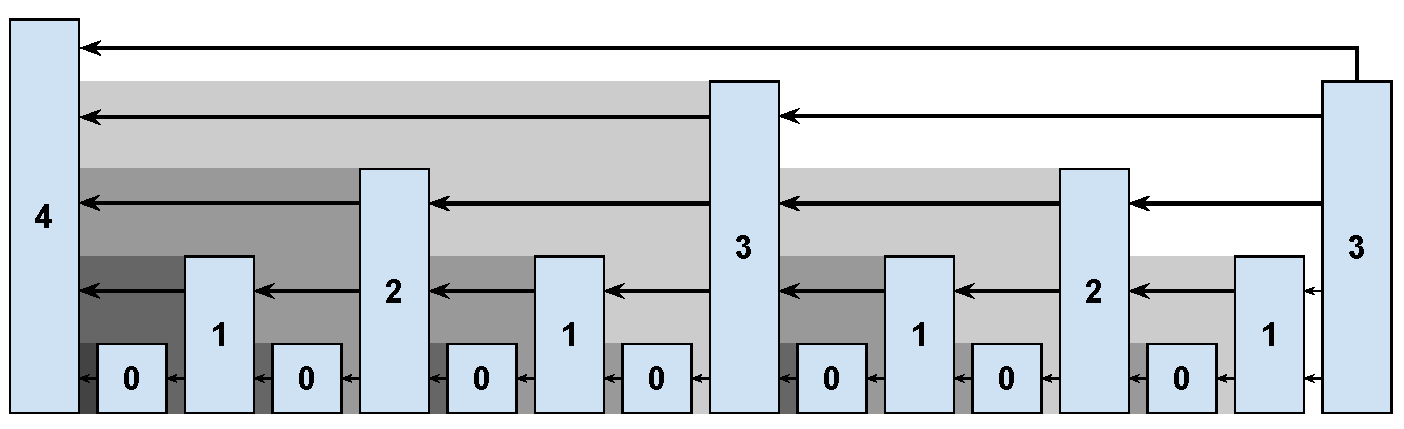
\includegraphics[width=0.9\columnwidth,keepaspectratio]{figures/level-shadows.pdf}
    \caption{The interlinked blockchain. Each superblock is drawn taller
    according to its achieved level. Each block links to all the blocks that are
    not being overshadowed by their descendants. The most recent (right-most)
    block links to the four blocks it has direct line-of-sight to.}
    \label{fig.hierarchy}
\end{figure}

The exact NIPoPoW protocol works like this: The prover holds a full chain
$\chain$. When the verifier requests a proof, the prover sends the last $k$
blocks of their chain, the suffix $\chi = \chain[-k{:}]$, in full. From the
larger prefix $\chain[{:}-k]$, the prover constructs a proof $\pi$ by selecting
certain superblocks as representative samples of the proof-of-work that took
place. The blocks are picked as follows. The prover selects the \emph{highest}
level $\mu^*$ that has at least $m$ blocks in it and includes all these blocks
in their proof (if no such level exists, the chain is small and can be sent in
full). The prover then iterates from level $\mu = \mu^* - 1$ down to $0$. For
every level $\mu$, it includes sufficient $\mu$-superblocks to cover the last
$m$ blocks of level $\mu + 1$, as illustrated in
Algorithm~\ref{alg.nipopow-prover}. Because the density of blocks doubles as
levels are descended, the proof will contain in expectation $2m$ blocks for each
level below $\mu^*$. As such, the total proof size $\pi \chi$ will be
$\Theta(m\log|\chain| + k)$. Such proofs that are polylogarithmic in the chain
size constitute an exponential improvement over traditional SPV clients and are
called \emph{succinct}.

\import{./}{algorithms/alg.nipopow-prover.tex}

Upon receiving two proofs $\pi_1\chi_1, \pi_2\chi_2$ of this form, the NIPoPoW verifier
first checks that $\lvert \chi_1 \rvert = \lvert \chi_2 \rvert = k$ and that
$\pi_1 \chi_1$ and $\pi_2 \chi_2$ form valid chains. To check that they are
valid chains, the verifier ensures every block in the
proof contains a pointer to its previous block inside the proof through either
the \emph{previd} pointer in the block header, or in the interlink vector. If
any of these checks fail, the proof is rejected. It then
compares $\pi_1$ against $\pi_2$ using
the $\leq_m$ operator, which works as follows. It finds the
lowest common ancestor block $b = (\pi_1 \cap \pi_2)[-1]$; that is, $b$ is the
most recent block shared among the two proofs. Subsequently, it
chooses the level $\mu_1$ for $\pi_1$ such that
$\lvert \pi_1\{b{:}\}\upchain^{\mu_1} \rvert \geq m$
(i.e., $\pi_1$ has at least $m$ superblocks of level $\mu_1$ following block
$b$) and the value
$2^{\mu_1} \lvert \pi_1\{b{:}\}\upchain^{\mu_1} \rvert$
is maximized.
It chooses a level $\mu_2$ for $\pi_2$ in the same fashion. The two proofs are
compared
by checking whether
$2^{\mu_1} \lvert \pi_1\{b{:}\}\upchain^{\mu_1} \rvert \geq
 2^{\mu_2} \lvert \pi_2\{b{:}\}\upchain^{\mu_2} \rvert$
and the proof with the largest score is deemed the winner. The comparison is
illustrated in Algorithm~\ref{alg.nipopow-maxchain}.

\import{./}{algorithms/alg.nipopow-maxchain.tex}

Blockchain protocols can be upgraded using hard or soft
forks~\cite{buterinforks}. In a \emph{hard fork}, blocks produced by
upgraded miners are not accepted by unupgraded miners. It is simplest to
introduce interlinks using a hard fork by mandating that interlink pointers are
included in additional fields in the block header. Unupgraded miners will not
recognize these fields and will be unable to parse upgraded blocks.
To ensure the block header is of constant size, instead of including all these
superblock pointers in the block header individually, they are organized into a
Merkle Tree of interlink pointers and only the root of the Merkle Tree is
included in the block header. In this case, the NIPoPoW prover that wishes to
show a block $b$ in their proof is connected to its more recently preceding
$\mu$-superblock $b'$, also includes a Merkle Tree proof proving that $H(b')$ is
a leaf in the interlink Merkle Tree root included in the block header of $b$.
The verifier has the additional job of verifying the veracity of these Merkle
inclusion proofs.

In a \emph{soft fork}, blocks created by unupgraded miners are not accepted by
upgraded miners, but blocks created by upgraded miners are accepted by
unupgraded miners. As such, any additional data introduced by the upgrade must
be included in a field that is treated like a comment by an unupgraded miner.
To interlink the chain via a soft fork, the interlink Merkle Tree root is
placed in the \emph{coinbase} transaction instead of the block header. Upgraded
miners include the correct interlink Merkle Tree root in their coinbase.
Upgraded miners receiving a new block validate that the interlink Merkle Tree
root is correct before accepting a block as valid. As this root can be
calculated in a deterministic manner from the previous blocks in the chain, it
can easily be validated. Unupgraded miners ignore this data and accept the block
regardless of whether it exists. The success of the fork depends on the majority
of the miner population upgrading. Whenever the NIPoPoW prover wishes to show that a
block $b$ in the proof contains a pointer to its most recently preceding
$\mu$-superblock $b'$, it must then accompany the block header of $b = s \conc
\overline{x} \conc ctr$ with the coinbase transaction $\coinbase$ of $b$ as well
as two Merkle Tree proofs: One proving that the coinbase transaction $\coinbase$
is in $\overline{x}$, and one proving that $H(b')$ is a leaf in the interlink
Merkle Tree whose root is included in $\coinbase$.


\section{The Chainsewing Attack}
\section{The Chainsewing Attack}\label{sec:attack}
We now make the critical observation that a thorny block can include interlink
pointers to blocks that are not its own ancestors in the $0$-level chain.
Because it must contain a pointer to the hash of the block it points to, they
must be older blocks, but they may belong to a
different $0$-level chain. This is shown in Figure~\ref{fig:false_interlink}.

\begin{figure}
	\begin{center}
		\iftwocolumn
			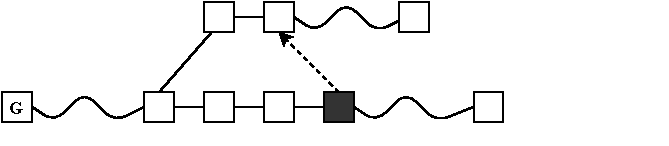
\includegraphics[width=0.6\columnwidth]{figures/false_interlink.pdf}
		\else
			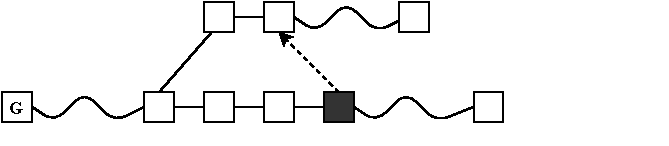
\includegraphics[width=0.35\columnwidth]{figures/false_interlink.pdf}
		\fi
	\end{center}
    \caption{A thorny block, colored black, in an honest party's chain, uses its interlink to point to a fork chain.}
	\label{fig:false_interlink}
\end{figure}

In fact, as the interlink vector contains multiple pointers, each pointer may
belong to a different fork. This is illustrated in
Figure~\ref{fig:thorny_block}. The interlink pointing to arbitrary directions
resembles a thorny bush.

\begin{figure}
	\begin{center}
		\iftwocolumn
			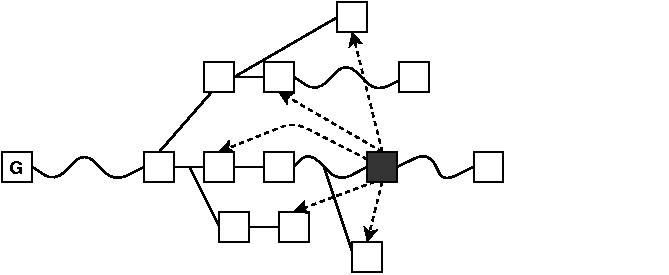
\includegraphics[width=0.5\columnwidth]{figures/thorny_block.pdf}
		\else
			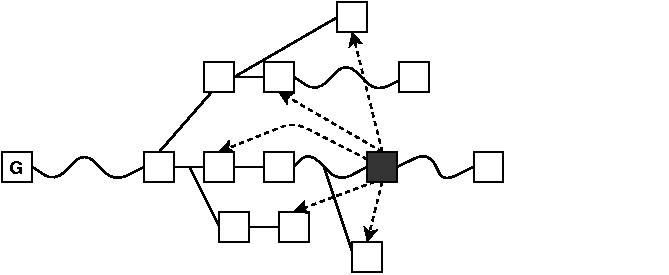
\includegraphics[width=0.4\columnwidth]{figures/thorny_block.pdf}
		\fi
	\end{center}
	\caption{A thorny block appended to an honest party's chain.
	The dashed arrows are interlink pointers.}
	\label{fig:thorny_block}
\end{figure}

We now present the \emph{chainsewing attack} against the na\"ive velvet NIPoPoW
protocol. The attack leverages thorny blocks in order to enable the adversary to
\emph{usurp} blocks belonging to a different chain and claim it as her own.
Taking advantage of thorny blocks, the adversary produces suffix proofs
containing an arbitrary number of blocks belonging to several fork chains. The
attack works as follows.

Let $\chain_B$ be a chain adopted by an honest party $B$ and $\chain_\mathcal{A}$, a fork of $\chain_B$ at some point, be maintained by the adversary. After the fork point $b = (\chain_B \cap \chain_\mathcal{A})[-1]$, the honest party produces a block extending $b$ in $\chain_B$ containing a transaction $\tx$. The adversary includes a conflicting (double spending) transaction $\tx'$ in a block extending $b$ in $\chain_\mathcal{A}$.
The adversary produces a suffix proof to convince the verifier that $\chain_\mathcal{A}$ is longer. In order to achieve this, the adversary needs to include a greater amount of total proof-of-work in her suffix proof, $\pi_\mathcal{A}$, in comparison to that included in the honest party's proof, $\pi_B$, so as to achieve $\pi_\mathcal{A} \geq_m \pi_B$. Towards this purpose, she miners intermittently on both $\chain_B$ and $\chain_\mathcal{A}$. She produces some thorny blocks in both chains $\chain_\mathcal{A}$ and $\chain_B$ which will allow her to usurp selected blocks of $\chain_B$ and present them to the light client as if they belonged to $\chain_\mathcal{A}$ in her suffix proof.

The general form of this attack for an adversary sewing blocks to one forked chain is illustrated in Figure~\ref{fig:generic_attack}. Dashed arrows represent interlink pointers of some level $\mu_\mathcal{A}$. Starting from a thorny block in the adversary's forked chain and following the interlink pointers, jumping between $\chain_\mathcal{A}$ and $\chain_B$, a chain of blocks crossing forks is formed, which the adversary claims as part of her suffix proof. Blocks of both chains are included in this proof and a verifier cannot distinguish the non-smooth pointers participating in this proof chain and, as a result, considers it a valid proof. Importantly, the adversary must ensure that any blocks usurped from the honest chain are not included in the honest NIPoPoW to force the NIPoPoW verifier to consider an earlier LCA block $b$; otherwise, the adversary will compete after a later fork point, negating any sewing benefits.

\begin{figure}
	\begin{center}
		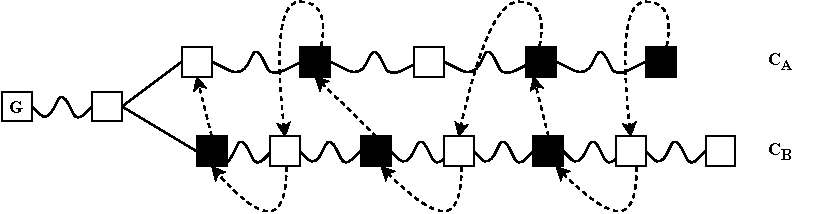
\includegraphics[width=0.9\columnwidth
		]{figures/generic_chainsewing_attack.pdf}
	\end{center}
	\caption{Generic Chainsewing Attack. $\chain_B$ is the chain of an honest party and $\chain_\mathcal{A}$ the adversary's chain. Thorny blocks are colored black. Dashed arrows represent interlink pointers included in the	adversary's suffix proof. Wavy lines imply one or more blocks.}
	\label{fig:generic_attack}
\end{figure}

This generic attack is made concrete as follows.
The adversary chooses to attack at some level $\mu_\mathcal{A} \in \mathbb{N}$ (ideally, if the honest verifier does not impose any succinctness limits, the adversary sets $\mu_A = 0$). As shown in Figure~\ref{fig:attack}, she first generates a block $b'$ in her forked chain $\chain_\mathcal{A}$ containing the double spend, and a block $a'$ in the honest chain $\chain_B$ which thorny-points to $b'$. Block $a'$ will be accepted as valid in the honest chain $\chain_B$ despite the invalid interlink pointers. The adversary also chooses a desired superblock level $\mu_B \in \mathbb{N}$ that she wishes the honest party to attain. Subsequently, the adversary waits for the honest party to mine and sews any blocks mined on the honest chain that are of level below $\mu_B$. However, she must bypass blocks that she thinks the honest party will include in their final NIPoPoW, which are of level $\mu_B$ (the blue block designated $c$ in Figure~\ref{fig:attack}). To bypass a block, the adversary mines her own thorny block $d$ on top of the current honest tip (which could be equal to the block to be bypassed, or have progressed further), containing a thorny pointer to the block preceding the block to be bypassed and hoping $d$ will not exceed level $\mu_B$ (if it exceeds that level, she discards her $d$ block). Once $m$ blocks of level $\mu_B$ have been bypassed in this manner, the adversary starts bypassing blocks of level $\mu_B - 1$, because the honest NIPoPoW will start including lower-level blocks. The adversary continues descending in levels until a sufficiently low level $\min\mu_B$ has been reached at which point it becomes uneconomical for the adversary to continue bypassing blocks (typically for a $1/4$ adversary, $\min\mu_B = 2$). At this point, the adversary forks off of the last sewed honest block. This last honest block will be used as the last block of the adversarial $\pi$ part of the NIPoPoW proof. She then independently mines a $k$-long suffix for the $\chi$ portion and creates her NIPoPoW $\pi \chi$. Lastly, she waits for enough time to pass so that the honest party's chain progresses sufficiently to make the previous bypassing guesses correct and so that no blocks in the honest NIPoPoWs coincide with blocks that have not been bypassed. This requires to wait for the following blocks to appear in the honest chain: $2m$ blocks of level $\mu_B$; after the $m^\text{th}$ $\mu_B$-level block, a further $2m$ blocks of level $\mu_B - 1$; after the $m^\text{th}$ such block, a further $2m$ blocks of the level $\mu_B - 2$, and so on until level $0$ is reached.

\begin{figure}
	\begin{center}
		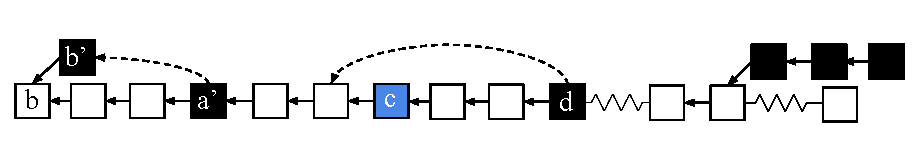
\includegraphics[width=0.99\columnwidth]{figures/chainsew-concrete.pdf}
	\end{center}
	\caption{A portion of the concrete Chainsewing Attack. The adversary's blocks are shown in black, while the honestly generated blocks are shown in white. Block $b'$ contains a double spend, while block $a'$ sews it in place. The blue block $c$ is a block included in the honest NIPoPoW, but it is bypassed by the adversary by introducing block $d$ which, while part of the honest chain, points to $c$'s parent. After a point, the adversary forks off and creates $k = 3$ of their own blocks.}
	\label{fig:attack}
\end{figure}

In this attack the adversary uses thorny blocks to ``sew'' portions of the
honestly adopted chain to her own forked chain. This justifies the name given to
the attack.
In order to make this attack successful, the adversary needs only to
produce few superblocks, while she can arrogate a large number of
honestly produced blocks. 
%Thus the attack succeeds with non-negligible probability.

We believe that the superlight-client protocol FlyClient\cite{flyclient} is also susceptible to Chainswewing attack under velvet fork conditions. 
We give insight for the velvet FlyClient attack in Appendix~\ref{sec:flyclient}.

%We illustrate simulation results for the success rate of our attack in Appendix~\ref{sec:simulation}. Our experiments find the attack with parameters $\mu_B = 10, \mu_A = 0, t = 1, n = 5, k = 15$ succeeds with a constant rate of success of approximately $0.26$, when the security parameter $m$ ranges from $3$ to $15$. This is in contrast to the best previously known attack (which does not make use of thorny blocks), which succeeds with probability less than $0.01$. Previous work recommends $m = 15$ for a $1/3$ adversary for a probability of failure bounded by $0.001$.


\section{Protocol Update}
In order to eliminate the Chainsewing Attack we propose an update to the velvet
NIPoPoW protocol. The core problem is that in her suffix proof the adversary
is able to claim not only blocks of forked chains,  which are in majority adversarially
generated due to the Common Prefix property, but also arbitrarily long parts of the
chain adopted by an honest player. Since thorny blocks are accepted as valid,
the verifier cannot distinguish blocks that actually belong in a chain from
blocks that only seem to belong in the same chain because they are pointed to
via a non-smooth pointer. \\


%% first reference to 1/3 adversary
\subsubsection{Honest Majority Assumption}
Compared to the typical setting of $1/2$-bounded adversary, the protocol we
propose requires stronger honest majority assumptions to be provably secure. 
In particular, our protocol is secure for adversary of total hashing power 
less than $1/2$ of the upgraded honest miners, meaning less than $1/3$ of the total number of miners generating blocks with interlinks. Therefore we define the Velvet Honest Majority assumption, which will be used in our security proof.

\begin{defn}{\textbf{Velvet Honest Majority}}
	\textit{Let $n_h$ be the number of upgraded honest miners. Then $t$ out of total $n$
	parties are corrupted such that $\dfrac{t}{n_h} < \dfrac{1 - \delta}{2} $. }
	\label{defn:velvet_honest_majority}
\end{defn}

We describe a protocol patch that operates as follows. The NIPoPoW protocol under velvet fork works as usual but each miner constructs smooth blocks. This means that  a block's interlink is constructed excluding thorny blocks. In this way, although thorny blocks are accepted in the chain, they are not taken into consideration when updating the interlink structure for the next block to be mined. No honest block could now point to a thorny superblock that may act as the passing point to the fork chain in an adversarial suffix proof. Thus, after this protocol update the adversary is only able to inject adversarially generated blocks from an honestly adopted chain to her own fork.
At the same time, thorny blocks cannot participate in an honestly
generated suffix proof except for some blocks in the proof's suffix $(\chi)$. This arguments holds because thorny blocks do not form a valid chain along with honestly mined blocks anymore. Consequently, as far as the blocks included in a suffix proof is concerned, we can think of thorny blocks as belonging in the adversary's fork chain for the $\pi$ part of the proof,  which is the comparing part between proofs. Figure 
\ref{fig:injection} illustrates this remark.\\

\begin{figure}[h!]
	\begin{center}
		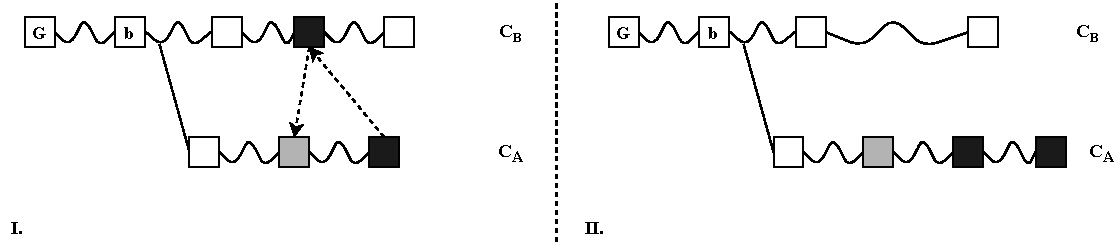
\includegraphics[scale=0.5]{figures/injection.png}
	\end{center}
	\caption{\textit{The adversarial fork chain $C_A$ and chain $C_B$ of an honest
	player. Thorny blocks are colored black. Dashed arrows represent interlink
	pointers. Wavy lines imply one or more blocks. When an adversarially generated
	block is sewed from $C_B$ into the adversary's suffix proof the verifier
	conceives $C_A$ as longer and $C_B$ as shorter.  \textbf{I:} The real picture
	of the chains. \textbf{II:} Equivalent picture from the verifier's perspective
	considering the blocks included in the corresponding suffix proof for each chain.}}
	\label{fig:injection}
\end{figure}


The protocol patch we suggest can be summarized as follows:\\


\subsubsection*{Protocol Patch for NIPoPows suffix proofs under velvet fork.} In order
to make NIPoPoWs safe under velvet fork conditions we suggest:
\begin{enumerate}
\item Strengthen the Honest Majority Assumption so that $t < \dfrac{1 - \delta}{2}n_h$,
where $n_h$ is the number of upgraded honest players.
%%% TODO: also provide short algorithm for the intrlink construction after the patch 
\item The NIPoPoW protocol under velvet fork works as usual but a miner constructs
a block's interlink without pointers to thorny blocks.
\end{enumerate}


The following Lemmas come as immediate results from the suggested protocol
update.\\

\begin{lemma}
	\textit{A velvet suffix proof constructed by an honest player cannot contain
	any thorny block.}
	\label{lemm:smooth_honest_suffix}
\end{lemma}

\begin{lemma} 
	\textit{Let $\mathcal{P_A} = (\pi_\mathcal{A}, \chi_\mathcal{A})$
	be a velvet suffix proof constructed by the adversary and block $b_s$, generated
	at round $r_s$, be the most recent smooth block in the proof. Then $\forall r:r < r_s$ no thorny blocks generated at round $r$ can be included in $\mathcal{P_A}$.}
	\label{lemm:smooths_before_smooth}
\end{lemma}
\textit{Proof.} By contradiction. Let $b_t$ be a thorny block generated at
some round $r_t < r_s$. Suppose for contradiction that $b_t$ is included in
the proof. Then, because $\mathcal{P_A}$ is a valid chain as for interlink
pointers, there exist a block path made by interlink pointers starting from $b_s$
and resulting to $b_t$. Let $b'$ be the most recently generated thorny block
after $b_t$ and before $b_s$ included in $\mathcal{P_A}$. 
Then $b'$ has been generated at a round $r'$ such that $r_t \leq r' < r_s$. Then
the block right after block $b'$ in $\mathcal{P_A}$ must be a thorny block since
it points to $b'$ which is thorny. But $b'$ is the most recent thorny block after
$b_t$, thus we have reached a contradiction.
\begin{flushright}
$\square$
\end{flushright}

\begin{lemma}
	\textit{Let $\mathcal{P_A} = (\pi_\mathcal{A}, \chi_\mathcal{A})$
	be a velvet suffix proof constructed by the adversary. Let $b_t$ be the oldest
	thorny bock included in $\mathcal{P_A}$ which is generated at round $r_t$. Then any block $b = \{b: b \in \mathcal{P_A} \wedge \text{b generated at }r \geq r_t \}$ is thorny.}
	\label{lemm:thorny_after_thorny}
\end{lemma}
\textit{Proof.} By contradiction. Suppose for contradiciton that $b_s$ is a smooth block generated at round $r_s > r_t$. Then from Lemma 
\ref{lemm:smooths_before_smooth} any block generated at round $r < r_s$ is smooth. But $b_t$ is generated at round $r_t < r_s$ and is thorny, thus we have reached a contradiction.
\begin{flushright}
$\square$
\end{flushright}

The following corollary emerges immediately from Lemmas 
\ref{lemm:smooths_before_smooth}, \ref{lemm:thorny_after_thorny}. This result is illustrated in Figure \ref{fig:adversarial_velvet_proof}.

\begin{corollary}
	\textit{Any adversarial proof $\mathcal{P_A} = (\pi_\mathcal{A}, \chi_\mathcal{A})$ containing both smooth and thorny blocks consists of a prefix smooth subchain followed by a suffix thorny subchain.}
	\label{cor:adversarial_proof_scheme}
\end{corollary}

\begin{figure}[h!]
	\begin{center}
		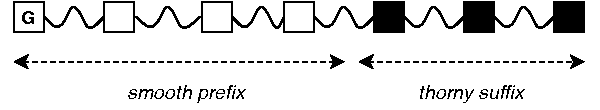
\includegraphics[scale=0.75]{figures/adversarial_velvet_proof.pdf}
	\end{center}
	\caption{\textit{In the general case the adversarial velvet suffix proof $\mathcal{P_A} = (\pi_\mathcal{A}, \chi_\mathcal{A})$ consists of an initial part of smooth blocks followed by thorny blocks.}}
	\label{fig:adversarial_velvet_proof}
\end{figure}

We now describe the algorithms needed by the upgraded miner, prover and verifier. The upgraded miner acts as usual except for including the interlink of the newborn block in the coinbase transaction. In order to construct an interlink containing only the smooth blocks, the miner keeps a copy of the ``smooth chain'' ($\mathcal{C}_S$) which consists of the smooth blocks existing in the original chain $\mathcal{C}$. The algorithm for extracting the smooth chain out of $\mathcal{C}$ is given in Algorithm 
\ref{alg:smooth_chain}. Function \textit{isSmoothBlock(B)} checks whether a
block \textit{B} is a smooth velvet by calling \textit{isSmoothPointer(B,p)}
for every pointer \textit{p} in \textit{B}'s interlink. Function
\textit{isSmoothPointer(B,p)} returns \emph{true} if $p$ is a valid 
pointer, in essence a pointer to the most recent \emph{smooth velvet}
for the level denoted by the pointer itself. The \textit{updateInterlink} algorithm is given in Algorithm \ref{alg:updateInterlink}, which is essentially the same as in the case of a hard/soft fork, except for working on the smooth chain $\mathcal{C}_S$ instead of $\mathcal{C}$.

\begin{algorithm}
	\SetAlgoNoLine
	\DontPrintSemicolon
	\SetKwProg{Fn}{function}{:}{\text{end function}}
	\Fn{smoothChain($\mathcal{C}$)}{
		$\mathcal{C}_S = \{ \mathcal{G} \}$\;
		$k \leftarrow 1$ \;
		\While{$\mathcal{C}[-k] \neq \mathcal{G}$}{
			\If{isSmoothBlock($\mathcal{C}[-k]$)}{
				$\mathcal{C}_S \leftarrow \mathcal{C}_S \cup \mathcal{C}[-k]$\;
			}
			$k \leftarrow k + 1$\;
		}
		return $\mathcal{C}_S$
	}
	\vspace{4mm}
	\Fn{isSmoothBlock(B)}{
		\If{$B = \mathcal{G}$}{
			\Return true\;
		}
 		\For{p $\in$ B.interlink} {
     		\If{$\neg$isSmoothPointer(B, p)}{
     			\Return false\;
     		}
 		}
 		\Return true\;
	}
	\vspace{4mm}
	\Fn{isSmoothPointer(B, p)}{
		$b \leftarrow Block(B.prevId)$\;
 		\While{b $\not =$ p} {
     		\If{$ level(b) \geq level(p) \wedge
     			\text{isSmoothBlock(b)} $}{
     			\Return false\;
     		}
     		\If{$b = \mathcal{G}$}{
     			\Return false\;
     		}
     		$b \leftarrow Block(b.prevId)$
 		}
		 \Return $\textit{isSmoothBlock(b)}$ \;
	}
 	\caption{Compute smooth chain}
 	\label{alg:smooth_chain}
\end{algorithm}

\begin{algorithm}[h!]
	\SetAlgoNoLine
	\DontPrintSemicolon
	\SetKwProg{Fn}{function}{:}{\text{end function}}
	\Fn{updateInterlinkVelvet($\mathcal{C}_S$)}{
		B' $\leftarrow \mathcal{C}_S[-1]$\;
		interlink $\leftarrow$ B'.interlink\;
 		\For{$\mu = 0$ to level(B')}{
 			interlink$[\mu]\leftarrow id(B')$
		 }
 		\Return interlink\;
	}
 	\caption{Velvet updateInterlink}
 	\label{alg:updateInterlink}
\end{algorithm}

The construction of the velvet suffix prover is given in Algorithm 
\ref{alg:velvet_suffix_prover}, which is essentially the same to that of a hard/soft fork except for working on smooth chain $\mathcal{C}_S$ instead of $\mathcal{C}$.

\begin{algorithm}[h!]
	\SetAlgoNoLine
	\DontPrintSemicolon
	\SetKwProg{Fn}{function}{:}{\text{end function}}
	\Fn{$ProveVelvet_{m,k}(\mathcal{C}_S$)}{
		$B \leftarrow \mathcal{C}_S[0]$\;
		\For{$\mu = \vert \mathcal{C}_S[-k].interlink \vert$ down to 0}{
			$\alpha \leftarrow \mathcal{C}_S[:-k] \{ B: \} \uparrow^\mu$\;
			$\pi \leftarrow \pi \cup \alpha$\;
			$B \leftarrow \alpha[-m]$\;
		}
		$\chi \leftarrow \mathcal{C}_S[-k:]$\;
		\Return $\pi\chi$
	}
 	\caption{Velvet Suffix Prover}
 	\label{alg:velvet_suffix_prover}
\end{algorithm}

\vspace{4mm}

In conclusion the Verify algorithm for the NIPoPoW suffix protocol remains the same as in the case of hard or soft fork.

After these changes the honest prover cannot contain any thorny blokcs in his suffix NIPoPow even if these blocks are part of $\mathcal{C}_B$. Therefore the adversary could try to supress honestly generated blocks in $\mathcal{C}_B$ in order to reduce the blocks that can represent the honest chain in a proof. In parallel, while the adversary mines suppressive thorny blocks on $\mathcal{C}_B$ she can still use her blocks in her NIPoPoW proofs, by chainsewing them. Consequently, even if a suppression attempt does not succeed, in case for example that a second honestly generated block is soon enough published, she does not drop the thorny block she generated but include it in her proof. 

More in detail, consider that the adversary wishes to attack a specific block level $\mu_B$ and generate a NIPoPow proof containing a block $b$ which contains a double spending transaction. Then she acts as follows. She may mine on her fork chain $\mathcal{C}_\mathcal{A}$ but when she observes a $\mu_B$-level block in $\mathcal{C}_B$ she mines a thorny block on $\mathcal{C}_B$ which jumps onto her fork chain, in order to suppress this $\mu_B$ block. If the suppression succeeds she has managed to damage the $\mu_B$ superchain and mine a block that she can afterwards use in her proof. If the suppression does not succeed she can still use the thorny in her proof. The above are illustrated in Figure \ref{fig:attack_after_update}.

\begin{figure}[h!]
	\begin{center}
    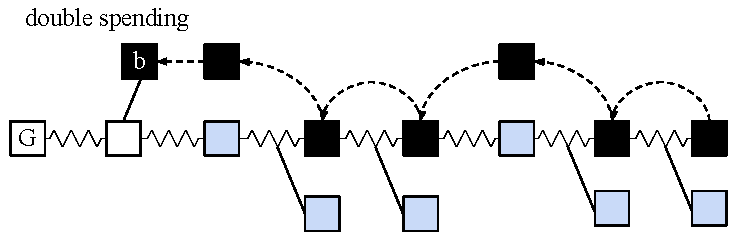
\includegraphics[scale=0.65]{figures/attack_after_update-crop.pdf}
	\end{center}
	\caption{\textit{The adversary suppress honestly generated blocks and chainsew thorny blocks in $\mathcal{C}_B$. Blue blocks are honestly generated blocks of a specific level of attack. The adversary tries to suppress them. If the suppression is not successful, the adversary can still use the block she mined in her proof.}}
	\label{fig:attack_after_update}
\end{figure}

\section{Combined Attack}
\section{Combined Attack}
After the suggested protocol update the honest prover cannot contain any thorny blokcs in his suffix NIPoPoW even if these blocks are part of his chain $\chain_B$. The adversary may exploit this fact as follows. She tries to suppress honestly generated blocks in $\chain_B$, in order to reduce the blocks that can represent the honest chain in a proof. In parallel, while she mines suppressive thorny blocks on $\chain_B$ she can still use her blocks in her NIPoPoW proofs, by chainsewing them. Consequently, even if a suppression attempt does not succeed, in case for example that a second honestly generated block is soon enough published, she does not lose the mining power spent but can still utilize it by including the block in her proof.

More in detail, consider that the adversary wishes to attack a specific block level $\mu_B$ and generate a NIPoPow proof containing a block $b$ of a fork chain which contains a double spending transaction. Then she acts as follows. She may mine on her fork chain $\chain_\mathcal{A}$ but when she observes a $\mu_B$-level block in $\chain_B$ she tries to mine a thorny block on $\chain_B$ in order to suppress this $\mu_B$ block. This thorny block contains an interlink pointer which jumps onto her fork chain. If the suppression succeeds she has managed to damage the $\mu_B$ superchain and, at the same time, to mine a block that she can afterwards use in her proof. If the suppression does not succeed she can still use the thorny block in her proof. The above are illustrated in Figure \ref{fig:attack_after_update}.

\begin{figure}[h!]
	\begin{center}
    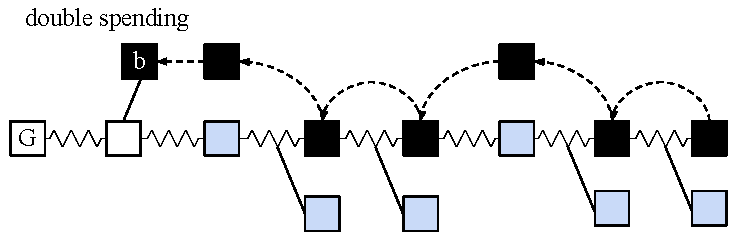
\includegraphics[width=0.95\columnwidth]{figures/attack_after_update-crop.pdf}
	\end{center}
	\caption{The adversary suppresses honestly generated blocks and chainsews thorny blocks in $\chain_B$. Blue blocks are honestly generated blocks of some level of attack. The adversary tries to suppress them. If the suppression is not successful, the adversary can still use the block she mined in her proof.}
	\label{fig:attack_after_update}
\end{figure}

The described attack consists a combined attack since both suppression and chainsewing are utilized. This combined attack forces us to consider the Velvet Honest Majority Assumption of (1/4)-bounded adversary, so as to guarantee that the unsuppressed blocks in $\chain_B$ suffice for constructing winning NIPoPoW proofs against the adversarial ones.

\section{Security Proof}
\begin{thm}{\textbf{Suffix Proofs Security under velvet fork}}
	Assuming honest majority under velvet fork conditions (\ref{defn:velvet_honest_majority}) such that $t \leq (1 - \delta) \dfrac{n_h}{2}$ where $n_h$ the number of upgraded honest players, the non-interactive proofs-of-proof-of-work construction for computable k-stable monotonic suffix-sensitive predicates under velvet fork conditions in a typical execution is secure.
\end{thm}
\textit{Proof.} By contradiction. Let $Q$ be a k-stable monotonic suffix-sensitive chain
predicate. Assume for contradiction that NIPoPoWs under velvet fork on $Q$ is insecure. Then, during an execution at some round  $r_3$, $Q(\mathcal{C})$ is defined and the verifier $V$ disagrees with some honest participant. $V$ communicates with adversary $\mathcal{A}$ and honest prover $B$. The verifier receives proofs $\pi_\mathcal{A}, \pi_B$ which are of valid structure. Because $B$ is honest, $\pi_B$ is a proof constructed
based on underlying blockchain $\mathcal{C}_B$ (with $\pi_B \subseteq \mathcal{C}_B$), which $B$
has adopted during round $r_3$ at which $\pi_B$ was generated. Consider
$\widetilde{\mathcal{C}}_\mathcal{A}$ the set of blocks defined as
$\widetilde{C}_\mathcal{A} = \pi_\mathcal{A} \cup \{ \bigcup \{\mathcal{C}_h^r\{:b_\mathcal{A}\}:  b_\mathcal{A} \in \pi_\mathcal{A}, \exists h,r : b_\mathcal{A} \in 
\mathcal{C}_{h}^{r}\}  \}$ where $\mathcal{C}_h^r$ the chain 
 that the honest player $h$ has at round $r$.

The verifier outputs $\neg Q(\mathcal{C}_B)$. Thus it is necessary that $\pi_\mathcal{A} {\geq}_m \pi_B$.
We show that $\pi_\mathcal{A} {\geq}_m \pi_B$ is a negligible event.

Let the levels of comparison decided by the verifier
be $\mu_\mathcal{A}$ and $\mu_B$ respectively. Let $b_0 = LCA(\pi_\mathcal{A}, \pi_B)$. Let $\mu'_B$ be the adequate level of proof
$\pi_B$  with respect to block $b_0$. Call $\alpha_\mathcal{A} = \pi_\mathcal{A} \uparrow^{\mu_\mathcal{A}}\{b_0:\}$,
$\alpha'_B = \pi_B \uparrow^{\mu'_B}\{b_0:\}$.

From Corollary \ref{cor:adversarial_proof_scheme} we have that the adversarial proof 
consists of a smooth interlink subchain followed by a thorny interlink subchain. We will refer to the smooth part of $\alpha_\mathcal{A}$ as $\alpha^{\mathcal{S}}_\mathcal{A}$ and to the thorny part as $\alpha^{\mathcal{T}}_\mathcal{A}$.   

%%%%%%%%   reconsider this paragraph
Our proof construction is based on the following intuition: we consider that $\alpha_\mathcal{A}$ consists of three distinct parts $\alpha_\mathcal{A}^1, \alpha_\mathcal{A}^2, \alpha_\mathcal{A}^3$ with the following properties. 

%$\vert  \alpha_\mathcal{A}^1 \vert = k_1, \vert \alpha_\mathcal{A}^2 \vert = k_2$ and $\vert \alpha_\mathcal{A}^3 \vert = k_3$. So $\vert \alpha_\mathcal{A} \vert = k_1 + k_2 + k_3$. Consider $\mathcal{S}_1, \mathcal{S}_2, \mathcal{S}_3$ the sets of consecutive rounds where the blocks of the three parts of $\alpha_\mathcal{A}$ are, respectively,  generated. 

Consider $b_0 = LCA(\pi_\mathcal{A}, \pi_B)$ the fork point between $\pi_\mathcal{A} \uparrow^{\mu_\mathcal{A}}, \pi_B \uparrow^{\mu_B}$ and $b_1 = LCA
(\alpha^{\mathcal{S}}_\mathcal{A}, \mathcal{C}_B)$ the fork point between $\pi^{\mathcal{S}}_\mathcal{A} \uparrow^{\mu_\mathcal{A}}, \mathcal{C}_B $ at the zero level as the honest prover could observe. Part
$\alpha_\mathcal{A}^1$ contains the blocks between $b_0$ exclusive and $b_1$ inclusive generated during the set of consecutive rounds $\mathcal{S}_1$ and $\vert  \alpha_\mathcal{A}^1 \vert = k_1$.
Consider $b_2$ the last block in $\alpha_\mathcal{A}$ generated by an honest player. Part $\alpha_{\mathcal{A}}^2$ contains the blocks between $b_1$ exclusive and $b_2$ inclusive generated during the set of consecutive rounds $\mathcal{S}_2$ and $\vert  \alpha_\mathcal{A}^2 \vert = k_2$. 
Consider $b_3$ the next block of $b_2$ in $\alpha_\mathcal{A}$. Then $\alpha_{\mathcal{A}}^3 = \alpha_\mathcal{A}[b_3:]$ and $\vert  \alpha_\mathcal{A}^3 \vert = k_3$ of all adversarially generated blocks generated during the set of rounds $\mathcal{S}_3$. So, $\vert \alpha_\mathcal{A} \vert = k_1 + k_2 + k_3$ and we will show that $\vert \alpha_\mathcal{A} \vert < \vert \alpha_B \vert$ .

The above are illustrated, among other, in Parts I, II of Figure \ref{fig:proof_velvet}.

\begin{figure}[h!]
	\begin{center}
    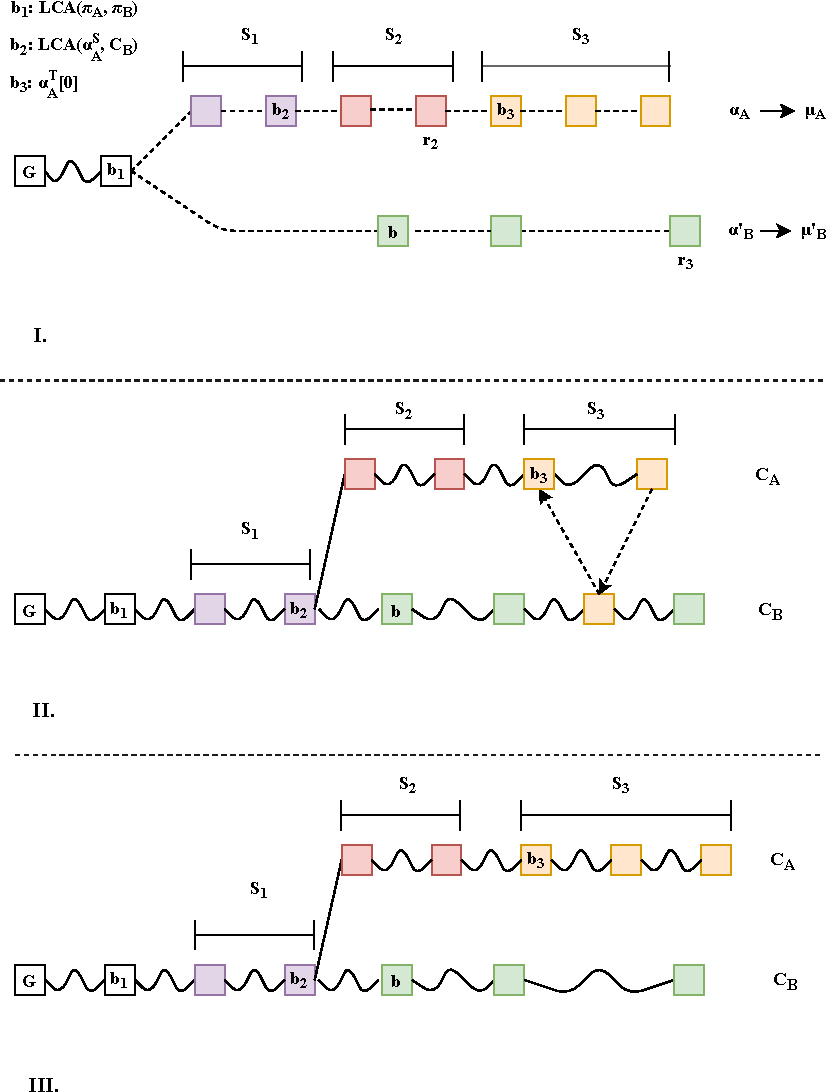
\includegraphics[scale=0.65]{figures/proof_velvet-crop.pdf}
	\end{center}
	\caption{\textit{ Wavy lines imply one or more blocks. Dashed lines and arrows imply
	interlink pointers to superblocks. \textbf{I}: the three round sets in two competing
	proofs at different levels, \textbf{II}: the corresponding 0-level blocks implied by the two proofs,
	\textbf{III}: blocks participating in chain $\mathcal{C}_B$ and block set $\widetilde{\mathcal{C}}_\mathcal{A}$ from the verifier's perspective.}}	
    \label{fig:proof_velvet}
\end{figure}

We will now show three successive claims under velvet fork conditions: First that $\alpha_\mathcal{A}^1$ contains only a few blocks. Second,  $\alpha_\mathcal{A}^2$ contains only a few blocks. And third,
the adversary is able to produce a winning $a_\mathcal{A}$ with negligible probability.\\

\textbf{Claim 1:} $\alpha_\mathcal{A}^1 = \alpha_\mathcal{A}(b_0 : b_1]$ contains only a few blocks. We have defined $b_0 = LCA(\pi_\mathcal{A}, \pi_B)$ and $b_1 = LCA
(\alpha^{\mathcal{S}}_\mathcal{A}, \alpha'_B \downarrow)$. First observe that there are no thorny blocks in $\alpha_\mathcal{A}^1$ since $\alpha_\mathcal{A}^1[-1] = b_1$ is a smooth block. This means that if $b_1$ was generated at round $r_{b_1}$ and $\alpha^{\mathcal{S}}_\mathcal{A}[-1]$ in round $r$, then $r \geq r_{b_1}$. So, $\alpha_\mathcal{A}^1$ consists a valid chain. We show the statement considering the two possible cases for the relation of $\mu_\mathcal{A}, \mu'_B$.

\textit{\underline{Claim 1a}:} If $\mu'_B \leq \mu_A$ then they are completely disjoint. In such a case of inequality, every block in $\alpha_A$ would also be
of lower level $\mu'_B$. Because of the adequate level $\mu'_B$ we know that $C\{b:\}\uparrow^{\mu'_B} = \pi\{b:\}\uparrow^{\mu'_B}$\cite{nipopows}. Subsequently, any block in $\pi_A\uparrow^{\mu_A}\{b:\}[1:]$ would also be included in proof $\alpha'_B$, but $b=LCA(\pi_A, \pi_B)$ so there can be no succeeding block common in $\alpha_A, \alpha'_B$.

\textit{\underline{Claim 1b}:} If  $\mu'_B > \mu_A$ then $\vert \alpha_A[1:]  \cap \alpha'_B\downarrow[1:] \vert = k_1 \leq g(2^{\mu'_B - \mu_A})$.\\
Let's call $b$ the first block in $\alpha'_B$ after block $b_0$.
Suppose for contradiction that $k_1 > g(2^{\mu'_B - \mu_A})$.  Since block $b$ of level $\mu'_B$ is also of level $\mu_A$, the adversary could include it in the proof but $b$ cannot exist in both $\alpha_A, \alpha'_B$ since $\alpha_A \cap \alpha'_B = \emptyset$ by definition. In case that the adversary chooses not to include $b$ in the proof then she can include no other blocks of $\mathcal{C}_B$ in her proof, since it would not consist a valid chain. Therefore, the adversary can include at most the $\mu_\mathcal{A}$ upgraded  blocks  between  $b_0$, $b$, which are expected to be equal to $g(2^{\mu'_B - \mu_A})$.

We conclude that
$\vert \alpha^{\mathcal{S}}_\mathcal{A} \cap \alpha'_B\downarrow[1:] \vert = k_{1} \leq g(2^{\mu'_B - \mu_\mathcal{A}})
$, where $g$ the velvet parameter denoting the percentage of upgraded honest parties.

Consequently, there are at least $\vert\alpha_\mathcal{A}\vert - k_1$
blocks after block $b$ in $\alpha_\mathcal{A}$ which are not honestly generated blocks existing in
$\mathcal{C}_B$. In other words, there are $\vert \alpha_\mathcal{A} \vert - k_1$
blocks after block $b$ in $\alpha_\mathcal{A}$, which are either thorny blocks existing in $\mathcal{C}_B$ either don't belong in $\mathcal{C}_B$.\\

\textbf{Claim 2.}
Part $\alpha_\mathcal{A}^2 = \alpha_\mathcal{A}(b_1:b_2]$ consists of only a few blocks. Let $ \vert \alpha_\mathcal{A}^2 \vert = k_2$.
We have defined $b_2 = \alpha_\mathcal{A}^2[-1]$ to be the last block generated by an honest player in $\alpha_\mathcal{A}$. Consequently no thorny block exists in $\alpha_\mathcal{A}^2$, so all blocks in this part belong in a proper zero-level chain $\mathcal{C}_\mathcal{A}^2$.  Let $r_{b_1}$ be the round at which $b_1$ was generated.
Since $b_1$ is the last block in $\alpha_\mathcal{A}$ which belongs in $\mathcal{C}_B$, then $\mathcal{C}_\mathcal{A}^2$ is a fork chain to $\mathcal{C}_B$ at some block $b'$ generated at round $r' \geq r_{b_1}$.

Let $r_2$ be the round when $b_2$ was generated by an honest party. Because an honest party has chain $\mathcal{C}_B$ at later round $r_3$ when the proof $\pi_B$ is constructed and because of the Common Prefix property on parameter $k_{2\downarrow} = g \cdot 2^{\mu_\mathcal{A}} \cdot k_2$, we conclude that $k_2 \leq k$, where $k$ is the Common Prefix parameter as defined in the Backbone series of papers\cite{backbone}.
% XXX: move definition of $k$ into preliminaries section

\textbf{Claim 3.} The adversary may submit a suffix proof such that $\alpha_\mathcal{A} \geq \alpha_B$
with negligible probability.
%%% @TODO: make formal arguments
As argued earlier the last $k_3$ blocks included in $\alpha_\mathcal{A}$ are all thorny blocks. In the worst case  all $k_3 $ blocks
are sewed from $\mathcal{C}_B$. This is the worst case scenario since each adversarially
generated block in $\mathcal{C}_B$ may have dropped one smooth block out of the chain
because of selfish mining. Considering this scenario, because of the strengthened
Honest Majority Assumption for $(1/3)$-bounded adversary, Theorem 3 for Chain
Quality guarantees that the majority of the blocks in $\mathcal{C}_B$ was computed by
honest parties, thus the honestly generated blocks in $\mathcal{C}_B$ for the same round
set sum to more amount of hashing power.\\
From all the above Claims we have that:\\
In the first round set, because of the common underlying chain:
\begin{equation} \label{eq_v_round_set_1}
2^{\mu_\mathcal{A}} \vert \alpha_\mathcal{A}^{k_1} \vert \leq 2^{\mu'_B} \vert \alpha'{_B^{k_1}} \vert
\end{equation}
Because of the adoption by an honest party of chain $\mathcal{C}_B$ at a later round $r_3$, we
have for the second round set:
\begin{equation} \label{eq_v_round_set_2}
2^{\mu_\mathcal{A}} \vert \alpha_\mathcal{A}^{k_2} \vert \leq 2^{\mu'_B} \vert \alpha'{_B^{k_2}} \vert
\end{equation}
In the third round set, because of good Chain Quality under the strengthened Honest
Majority Assumption and Theorem 3 we have:
\begin{equation} \label{eq_v_round_set_3}
2^{\mu_\mathcal{A}} \vert \alpha_\mathcal{A}^{k_3} \vert < 2^{\mu'_B} \vert \alpha'{_B^{k_3}} \vert
\end{equation}
Consequently we have:

\begin{equation*}
2^{\mu_\mathcal{A}} ( \vert \alpha_\mathcal{A}^{k_1} \vert + \vert \alpha_\mathcal{A}^{k_2} \vert + \vert
\alpha_\mathcal{A}^{k_3} \vert ) < 2^{\mu'_B} ( \vert \alpha'{_B^{k_1}} \vert + \vert
\alpha'{_B^{k_2}} \vert + \vert \alpha'{_B^{k_3}} \vert) \Rightarrow
\end{equation*}

\begin{equation} \label{eq_v_all_round_sets}
2^{\mu_\mathcal{A}} \vert \alpha_\mathcal{A} \vert < 2^{\mu'_B} \vert \alpha'{_B} \vert
\end{equation}

Therefore we have proven that $2^{\mu'_B} \vert \pi_B \uparrow^{\mu'_B} \vert >
2^{\mu_\mathcal{A}} \vert \pi_\mathcal{A}^{\mu_\mathcal{A}} \vert$. From the definition of $\mu_B$, we know
that $2^{\mu_B} \vert \pi_B \uparrow^{\mu_B} \vert > 2^{\mu'_B} \vert \pi_B
\uparrow^{\mu'_B} \vert$ because it was chosen $\mu_B$ as level of comparison
by the Verifier. So we conclude that $2^{\mu_B} \vert \pi_B \uparrow^{\mu_B}
\vert > 2^{\mu_\mathcal{A}} \vert \pi_\mathcal{A} \uparrow^{\mu_\mathcal{A}} \vert$.

\begin{flushright}
$\square$
\end{flushright}

%\appendix

%\section{Location}
%Note that in the new ACM style, the Appendices come before the References.

\begin{acks}
% TODO: For the submission, don't include acknowledgments since they would most likely deanonymize you.
\end{acks}


\bibliographystyle{ACM-Reference-Format}
\bibliography{refs}

\end{document}
